\documentclass{article}
\usepackage[utf8]{inputenc}

\usepackage{float}
\usepackage{natbib}
\usepackage{graphicx}
\usepackage[export]{adjustbox}
\usepackage{multirow}
\usepackage{hyperref}
\usepackage{titlesec}
\usepackage{ragged2e}



\begin{document}
\title{COS301 Team Gamma: Integration Team Goals}
\begin{figure}
    \centering
    
\includegraphics[width=\textwidth]{logo.png}
\end{figure}
\date{March 2020}

\maketitle

\section{Introduction}
This document describes the responsibilities and all deliverables for the \\Integration Team.
\\ \\
Demo \#1 Due Date: Thursday 12 March 20:00
\newpage

\section{Organisation}
\subsection{ClickUP}
You need to elect a team leader if you have not done so already. Work together with this member to create tasks and sub-tasks for each member in your team on \url{http://clickup.com} (on the COS301 workspace you have been invited to). \\

\begin{figure}[h]
    \centering
    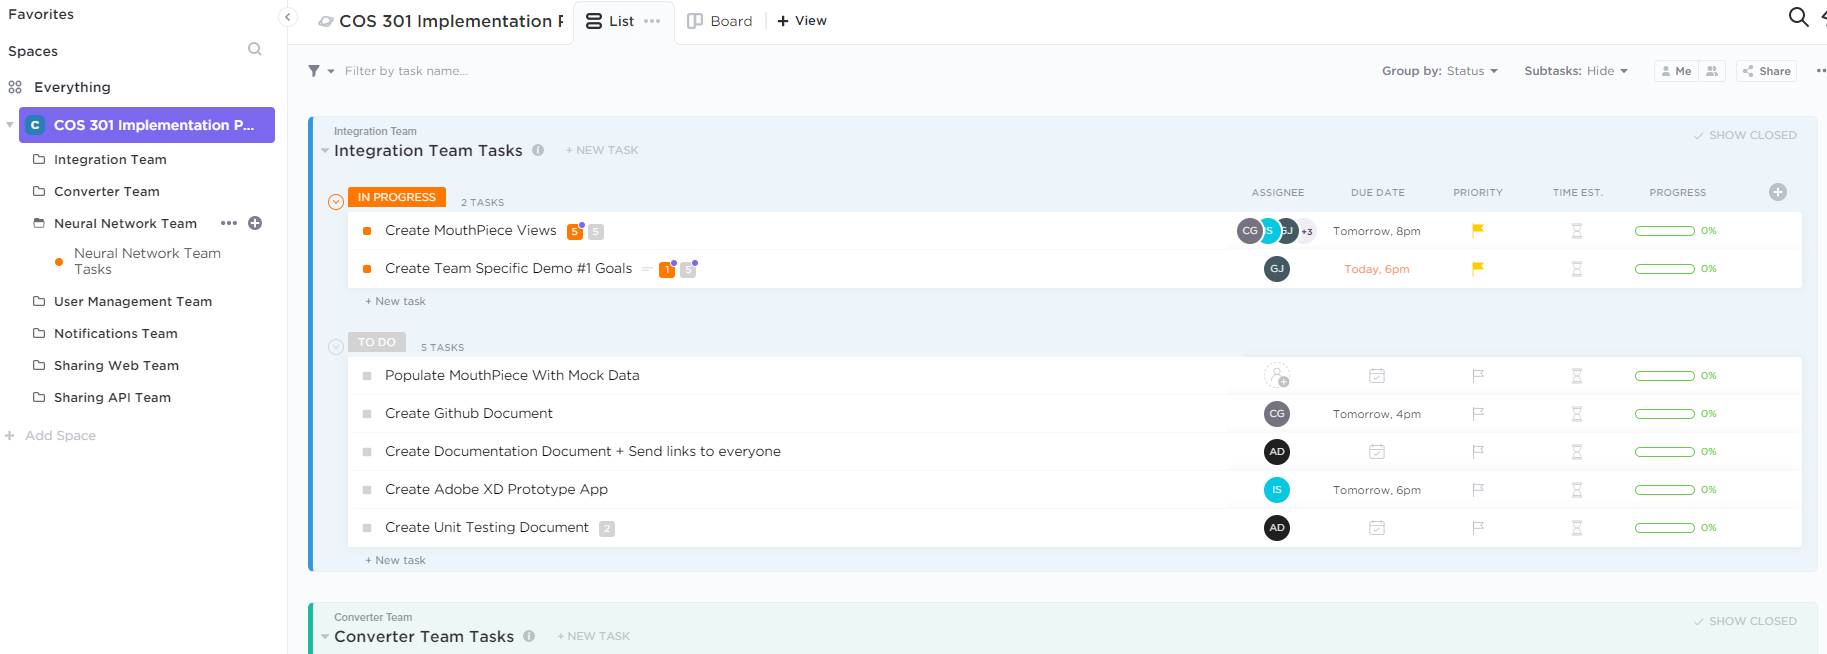
\includegraphics[width=\textwidth]{clickup.png}
\end{figure}

Ensure that you indicate progress and mark tasks as complete. This page will be displayed at the demo.

\subsection{Slack}
Although we have created a WhatsApp group - we do still find it easier for in-group discusions to happen on the slack channels. Simply login to \url{http://cos-301.slack.com}

\newpage

\section{Overall Team Tasks}
These are the tasks to be done by your team for the final product (not specifically Friday's demo).

\begin{itemize}
    \item Android app (in Flutter)
    \item Register user
    \item Login user
    \item Update user preferences
    \item List available mouth packages
    \item Search available mouth packages
    \item Download mouth packages to device storage

\end{itemize}

\vspace{1cm}

\begin{center}
   \textit{The tasks are always subject to change, but we have tried our utmost best to sketch out the entire project ahead.}
\end{center}

\newpage


\section{Team Tasks for Friday}

\subsection{Documentation}
\textbf{All documentation to be created in Overleaf}

\subsubsection{System Plan}
Implement and explain how the entire team Gamma will function together including:

\begin{itemize}
    \item Project management system (ClickUP)
    \item Collaborative communication platform (Slack)
    \item Decide on the technologies and deployment of the entire system
    \item Setup documents for each individual team explaining their tasks
\end{itemize}

\subsubsection{Frameworks}
You are required to do some research on frameworks that you could implement to assist your \textbf{Overall Team Tasks}. Write a short report on only the frameworks that you are keen to implement. Show its benefits and how you can implement it with the existing technologies. \\

\textbf{Some examples}
\begin{itemize}
    \item \url{https://flutter.dev/}
    \item \url{https://pub.dev/packages/http}
\end{itemize}

\subsection{Development Environment}
You are required to setup the development environment (have it running on at least one member's device, ready to demo). Setup everything you think you require. \\
\newline
\textbf{At bear minimum}
\begin{itemize}
    \item Android Studio
    \item Visual Studio Code
    \item Flutter
\end{itemize}

\begin{center}
   \textit{This is required for your implementation in any case.}
\end{center}

\newpage

\subsection{Implementation}
You are required to design and implement each view of the Android app in Flutter. \\

\textbf{These views include:}
\begin{itemize}
    \item Choose Listening Mode
    \item Login and Registration
    \item Select Mouth
    \item Voice Training Start Listening
    \item Profile
    \item Listening Mode Activated
    \item Home
    \Item Collection of Mouth Packs
    \Item Search
\end{itemize}

The views will be demoed live.

\subsubsection{Unit Testing}
Describe how your team will implement unit testing. Better yet - implement it in the Demo where possible.


\end{document}